\chapter{Developed Homography Ranking Method}
\label{chap:HomographyRanking}

This chapter is dedicated to one of our experiments that were not completely related to the \gls{vot} itself, yet we achieved an original scientific contribution that could potentially be applied to object tracking. Even though we did not continue with the homography-based object tracking due to limitations of available datasets, still we would like to elaborate on our developed approach. The proposed method was fully described as well as scrupulously tested under difficult conditions. The write-up of the whole research process was eventually published in a journal~\cite{ondrasovic2021homography}, building on top of a conference article~\cite{ondrasovic2020foundations}.

\section{Introduction}
\label{sec:HomographyIntroduction}

Computer vision often deals with diverse image transformations to improve the outcome of the subsequent post-processing phase. The perspective transformation was deemed of particular interest to our goal of traffic analysis. Specifically, removal of perspective distortion. To this end, the so-called homography mapping is often exploited.

Broadly speaking, homography is a perspective projection of a plane from one camera view into a different camera view. The perspective projection maps points from a $3$D world onto a $2$D image plane along lines that emanate from a single point~\cite{geetha2013automatic, bousaid2020perspective}. Such a projection is contained within a $3 \times 3$ invertible transformation matrix called the homography matrix (or just homography) with $8$ \gls{dof}. A general homography matrix can be defined as follows
\begin{equation}
    \label{eq:HomographyMatrix}
    \H =
    \begin{bmatrix}
        h_{11} & h_{12} & h_{13} \\
        h_{21} & h_{22} & h_{23} \\
        h_{31} & h_{32} & h_{33}
    \end{bmatrix}
\end{equation}
This transformation may facilitate mapping between two views of the same plane. Concretely, a single vector $\vectt{u}{u_x, u_y, 1}$, which represents a warped keypoint in homogeneous coordinates, is mapped onto the rectified keypoint $\vectt{\tilde{u}}{\tilde{u}_x, \tilde{u}_y, 1}$, by the homography $\H$ using the transformation $s \vect{\tilde{u}} \approx \H \vect{u}$, where $s$ represents the scale factor. In our case, the goal was to rectify the image so that it looks as if the camera was in an orthogonal position with respect to the desired plane in the world.

Homography is frequently adopted for text document rectification to generate a fronto-parallel view~\cite{lu2005perspective, miao2006perspective}, image stitching~\cite{adel2014image, gao2011constructing}, extracting metric information from $2$D images~\cite{zhang2000flexible}, pose estimation~\cite{mariyanayagam2018poseestim}, and for various traffic-related applications, \egtext{}, ground-plane detection~\cite{arrospide2010homography}, and bird's-eye view projection~\cite{luo2010low}.

We aimed at exploring the possibility of employing homography for \gls{vot}. The primary incentive was the fact that as long as a static camera is used and a few assumptions that we will discuss later hold, the scene may be easily stripped off the effect of the perspective distortion. Consequently, the use case of tracking vehicles visually using a static camera while exploiting a fronto-parallel view over the road seemed like a plausible extension with possible advantages for traffic analysis. Furthermore, the combination of homography and object tracking is present in the literature, \egtext{}~\cite{bose2004groundplane, zhang2012homographytrack, Mei2009}. Bose~\etal{}~\cite{bose2004groundplane} presented a fully automated technique for both affine and metric rectification of a given ground plane by simply tracking moving objects. The derivation of the necessary constraints for projective transformation between the image and the ground plane was obtained by observing objects that moved at constant velocity in the world for some part of their trajectory. We conjectured that the extra information about the scene geometry that we may achieve using rectification could aid in making the tracking more accurate. Visual trackers are often supported by motion models such as Kalman filter~\cite{kalman1960linearfilter}, so the rationale was to estimate the motion model in an orthogonal projection, rather than a perspectively distorted one.

% ------------------------------------------------------------------------------
\begin{figure}[t]
    \centerline{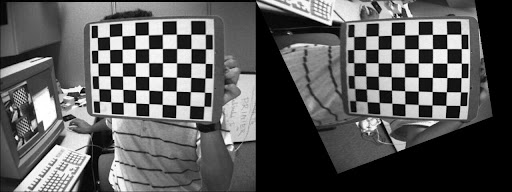
\includegraphics[width=0.8\linewidth]{figures/homography/chessboard_marker.jpg}}
    \caption[Chessboard marker]{An example of a chessboard marker present in a scene that may be used to establish a point correspondence that would serve for a homography transformation. The rectified, fronto-parallel view demonstrates the desired effect that points present on the ``ground'' plane are properly projected, whereas other points suffer from substantial distortion. \externalsrc{\cite{webhomographybasiccode}}}
    \label{fig:ChessboardMarker}
\end{figure}
% ------------------------------------------------------------------------------

% ------------------------------------------------------------------------------
\begin{figure}[t]
    \centerline{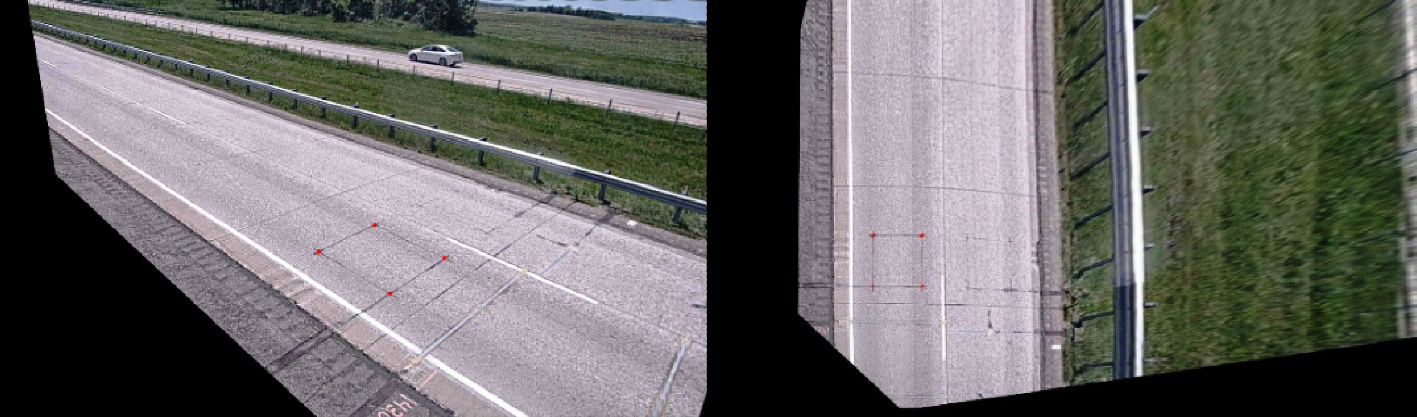
\includegraphics[width=\linewidth]{figures/homography/homography_road.png}}
    \caption[Square marker on a road]{An example of a virtual square marker present on a road that may be used to establish a point correspondence, and thus the homography transformation, too. The obtained view allows for many applications such as speed and size measurements that would otherwise be a lot more problematic in a perspectively deformed view. \externalsrc{\cite{bose2004groundplane}}}
    \label{fig:RoadMarker}
\end{figure}
% ------------------------------------------------------------------------------

A common approach to estimate the homography is to use a set of at least four $2$D point correspondences~\cite{hartley1997defense}. The points that are used for establishing the $2$D point correspondences will be referred to as keypoints. These keypoints may belong to a marker which is an object with a known shape that is either naturally occurring or artificially positioned in the scene. A regular, easy-to-detect pattern (\egtext{}, a chessboard) is commonly utilized~\cite{zhang2016flexible} (\figtext{}~\ref{fig:ChessboardMarker}). A single marker is identified in the image by multiple independent keypoints that have a direct correspondence to its real shape, thus making a group of point correspondences. For the sake of traffic analysis, the marker may be represented by virtually any points on the image as long as certain conditions are met (\figtext{}~\ref{fig:RoadMarker}). However, the point correspondences established this way are often subjected to noise, thus errors may be introduced in the homography estimation. Although $4$ keypoints are satisfactory, often a greater number of keypoints is used, allowing to use optimization to minimize a suitable cost function~\cite{osuna2016multiobjective, mou2013robust}. Subsequently, an outlier removal becomes an important step in the processing pipeline, for which effective and robust algorithms such as RANSAC~\cite{fischler1981ransac} are usually employed.

% ------------------------------------------------------------------------------
\begin{figure}[t]
    \centerline{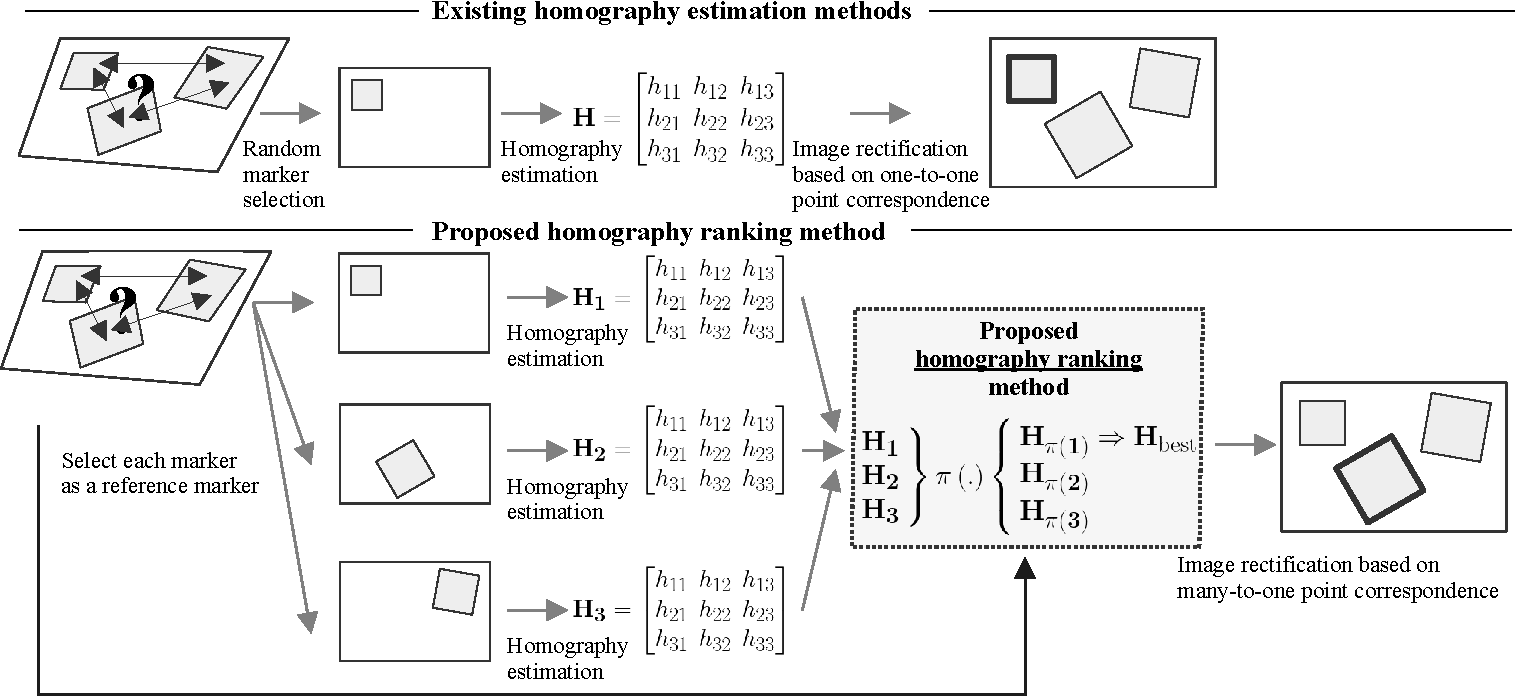
\includegraphics[width=\linewidth]{figures/homography/motivation_diagram.pdf}}
    \caption[Homography ranking motivation diagram]{A fundamental difference between existing homography estimation methods and our proposed method for homography ranking. If there are multiple markers while the information about their relative positions in the world is absent, the existing approaches can only estimate isolated homographies without the ability to select the best one. To address this issue, our method easily serves as an extension to existing approaches by exploiting multiple markers to rank the isolated homographies from the ``best'' to the ``worst''.}
    \label{fig:HomographyMotivationDiagram}
\end{figure}
% ------------------------------------------------------------------------------

A real-world application of generating a bird's-eye view over a road from a video recording when we could not use a large marker to cover a sufficient portion of the road (\figtext{}~\ref{fig:MultipleMarkersOnRoad}) motivated this entire project. We observed that, under our conditions, the homography estimation based on a single small marker was inaccurate. Therefore, there was an attempt to utilize multiple small markers and measure their relative positions. However, as is often the case in practice, their position measurements were highly noisy at best. Thus, we had to bypass the position measurements altogether, which led us to adopt the proposed method, instead. It is crucial to emphasize that our method can also be adopted in a situation when the marker placed at various positions on the same planar surface can be seen at different frames using a static camera. Stacking the captured frames onto each other would effectively yield an artificially generated view of multiple markers.

Assume a presence of a sole marker in the scene (\figtext{}~\ref{fig:RoadMarker}). Moreover, assume the view of the marker is perspectively distorted. If we know its real shape, then it is possible to compute the homography. However, when multiple copies of the same marker are visible, but their positions in the world are unknown, the detailed information about the shape is not enough to incorporate all the keypoints in the estimation. In the absence of position information, existing approaches for homography estimation based on point correspondences do not work because the projection has to preserve the proportional positions. As a result, estimating the homography while not knowing the ground-truth layout of the keypoints up to an arbitrary scale does not guarantee, and often does not even lead, to the correct result.

Under the constraints discussed above, the existing methods can only generate an isolated homography for each marker based on the one-to-one point correspondence (\figtext{}~\ref{fig:HomographyMotivationDiagram}). Each homography may be affected by different sources of noise, \egtext{}, low resolution, blur, or keypoint detection. Thus, the outcome of rectification may vary up to a great extent. In addition, many practical applications often use a marker that just covers a small portion of the image, increasing susceptibility to noise as a result. The trivial solution would be to use a bigger marker that covers the majority of the estimated plane's area. But such a solution is often cumbersome. It is simply not possible to ``merge'' multiple isolated homographies together.

% ------------------------------------------------------------------------------
\begin{figure}[t]
    \centerline{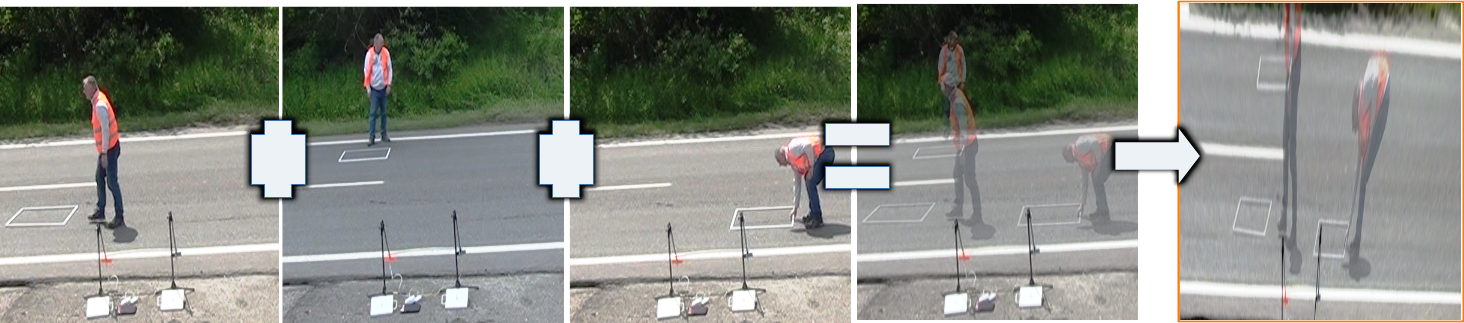
\includegraphics[width=\linewidth]{figures/homography/markers_on_the_road.png}}
    \caption[Multiple markers on the road]{A motivating real-world example. We can see different frames captured during a video recording that show various positions of the same marker. The picture after the ``equality'' sign is a merge of the previous frames for better illustration. Due to the use of a static camera, we may treat the positions of the given marker on individual frames as if they were captured simultaneously. However, the question remains unanswered. Given multiple markers in the absence of their position information, which one is the best to choose for rectification?}
    \label{fig:MultipleMarkersOnRoad}
\end{figure}
% ------------------------------------------------------------------------------
\section{Preliminaries}
\label{sec:HomographyPreliminaries}

This section contains a description of our custom terminology. Despite the existence of standard conventions for naming certain aspects of our problem, we nevertheless had to coin a few more terms for clarity.

We define a marker as an object with a known, easy-to-detect shape. Such object can be either naturally occurring or artificially placed on the planar surface of the scene we want to remove perspective distortion from, i.e., to produce a bird's-eye view. The marker contains keypoints, which is a set of distinct, independent, visual feature points (for instance, corners). The chosen keypoints visible in the perspectively deformed image are called the \mbox{warped keypoints}. The set of the \mbox{rectified keypoints} is represented in the desired image (not subjected to perspective distortion) and is produced from the warped keypoints using the homography projection. Last but not least, the \mbox{point correspondence} is a relationship between the warped and the \mbox{target keypoints} and it is necessary for homography estimation. In an ideal case, the rectified keypoints match the target keypoints in terms of their pixel positions (see \figstr{}~\ref{fig:HomographyTerminology}).

% ------------------------------------------------------------------------------
\begin{figure}[t]
    \centering
    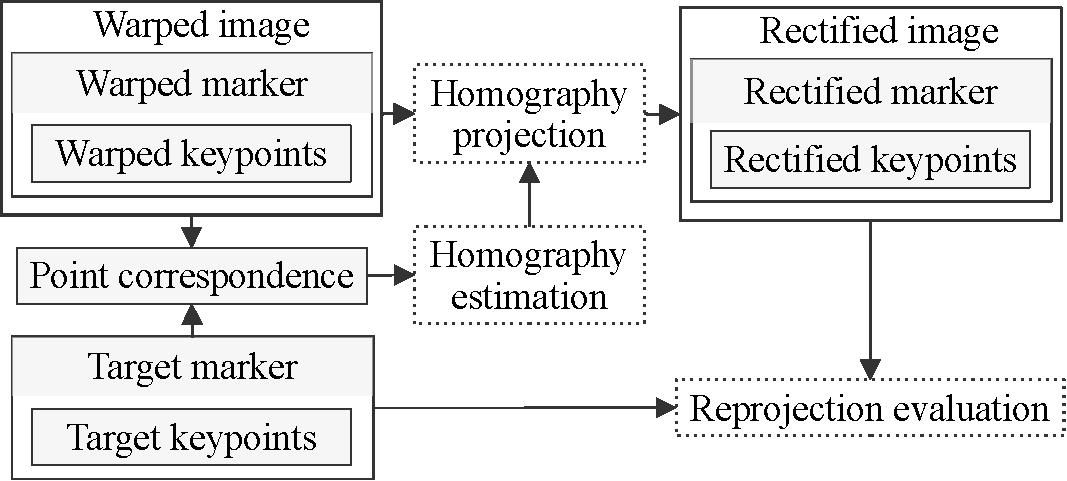
\includegraphics[width=0.6\linewidth]{figures/homography/terminology.pdf}
    \caption[Homography ranking terminology]{Visualization of relationships within our established terminology. This diagram also depicts the hierarchical dependence between individual terms. In addition, the dotted elements represent processes with arrows denoting their input and output.}
    \label{fig:HomographyTerminology}
\end{figure}
% ------------------------------------------------------------------------------

Unless stated otherwise, a \mbox{\textbf{similarity transformation}} denotes a limited affine transformation with $4$ DoF which encompasses translation, rotation and uniform scaling (equation \ref{eq:SimilarityMatrices}). Specifically, let $\mset{K}_1$ and $\mset{K}_2$ be sets of feature keypoints belonging to objects $O_1$ and $O_2$. We refer to the objects $O_1$ and $O_2$ as \mbox{\textbf{similar}} if there exists a similarity transformation $\psi$, such that $\mset{K}_1 = \func{\psi}{\mset{K}_2}$ and $\mset{K}_2 = \func{\psi^{-1}}{\mset{K}_1}$. For instance, $O_1$ and $O_2$ may represent rectangles of different sizes whilst having a equal aspect ratio.

Let $m$ denote the number of markers and $k$ represent the number of keypoints belonging to each marker in consideration. We describe each $i$-th marker using a $3 \times k$ matrix $\suprbrackets{\mtx{W}}{i}$ that stores the warped keypoints as
\begin{equation}
    \suprbrackets{\mtx{W}}{i} =
    \begin{bmatrix}
        \subsuprbrackets{x}{1}{i} & \subsuprbrackets{x}{2}{i} & \dots & \subsuprbrackets{x}{k}{i} \\
        \subsuprbrackets{y}{1}{i} & \subsuprbrackets{y}{2}{i} & \dots & \subsuprbrackets{y}{k}{i} \\
        1                         & 1                         & \dots & 1
    \end{bmatrix},
    i = 1, \dots, m.
\end{equation}
Analogivally, we describe the target keypoints using a $3 \times k$ matrix $\mtx{T}$. Owing to the many-to-one point correspondence, only one specification is sufficient. Just beware that the ordering of keypoints had to match the warped keypoints defined above, so
\begin{equation}
    \mtx{T} =
    \begin{bmatrix}
        \tilde{x}_1 & \tilde{x}_2 & \dots & \tilde{x}_k \\
        \tilde{y}_1 & \tilde{y}_2 & \dots & \tilde{y}_k \\
        1           & 1           & \dots & 1
    \end{bmatrix},
\end{equation}
with the point correspondence relationship formulated as
\begin{equation}
    \subsuprbrackets{x}{j}{i} \simeq \tilde{x}_j, \subsuprbrackets{y}{j}{i} \simeq \tilde{y}_j, i = 1, \dots, m, j = 1, \dots, k.
\end{equation}

\chapter{Methodology}
\label{chap:Methodology}

In this chapter, we describe our scientific constributions. We start off with our attempts that did not manifest into primary advances in the field of object tracking per set, yet they were significant enough that they earned a journal publication in the end. Subsequently, we dive into our contributions to the field of Siamese-based \gls{vot}, which is the primary goal of this dissertation thesis.

\section{Homography and Visual Object Tracking}
\label{sec:HomographyAndVisualObjectTracking}


\section{Experiments and Discussion}
\label{sec:HomographyExperiments}

The evaluation of the proposed homography ranking algorithm involved various conditions. We tested cases that included diverse similarity transformations applied to original markers as well as noisy point correspondence, \egtext{}, errors in marker detection since these are the expected problems in real-world scenarios.

\figtext{}~\ref{fig:HeatmapsBestWorst} demonstrates how the reprojection error varies with respect to the marker position. It can be observed that the marker position can be approximately estimated by looking at the heatmap which represents the pixel-wise reprojection error over the image. However, the important property is that not all markers are subjected to the same pattern of error variation. This is the core observation that motivated our solution in the first place. The objective is to select the marker that minimizes the pixel-wise reprojection error within the region of the image that is as broad as possible. That is why we evaluate our method by computing the reprojection error over each pixel, not just the keypoints. The rationale is that subsequent image postprocessing would greatly benefit from having the area of the image as large as possible that is reprojected properly.

% ------------------------------------------------------------------------------
\begin{figure}[t]
    \centerline{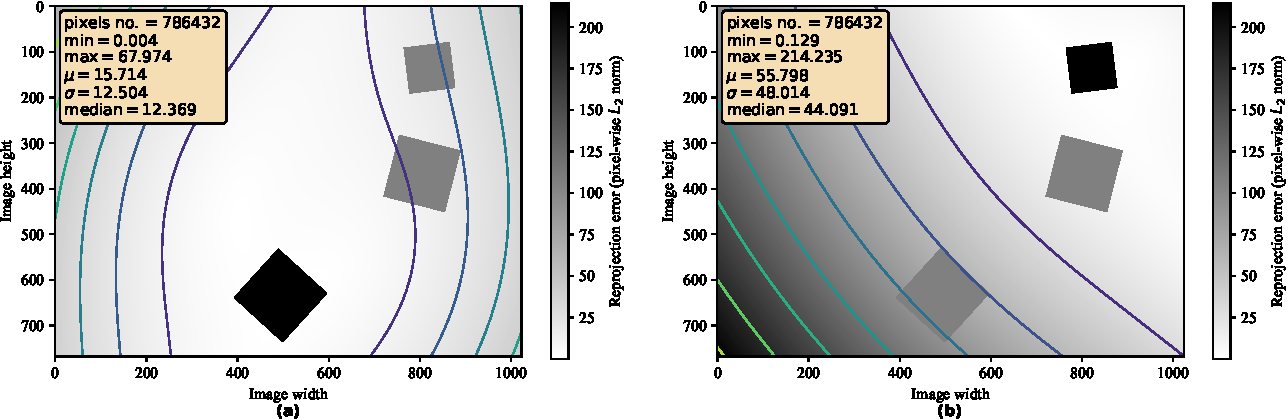
\includegraphics[width=\linewidth]{figures/homography/heatmaps_best_worst.pdf}}
    \caption[Homography ranking heatmaps]{Distribution of pixel-wise reprojection error. The heat map along with the corresponding contours demonstrate the varying distance between the ground truth and rectified pixel position after removing the perspective distortion. The bold square represents the reference marker. We show the result of \imgpartdesc{a} the ``best'' marker and \imgpartdesc{b} the ``worst'' marker. This test scenario includes all similarity transformations as well as noise in point correspondence.}
    \label{fig:HeatmapsBestWorst}
\end{figure}
% ------------------------------------------------------------------------------

All the test scenarios indicated the following trend. On average, the homography with the highest score improved the relative performance to the baseline performance the most (both median and mean above $60$\%). The lowest-ranked homography often led to significantly worse performance (median and mean around $-90$\%). These values varied moderately across different setups.

\subsubsection{Implementation Details}
\label{sssec:HomographyImplementation}

Our proposed algorithm can be utilized to extend any homography estimation method that exploits point correspondences. To demonstrate, we adopted time-tested implementations from the \opencv{}~$4.4.0$ library~\cite{bradski2008learning}. Each homography was estimated by the \srcfuncname{findHomography} function which internally employs DLT~\cite{abdel2015direct} algorithm for $k = 4$ and RANSAC~\cite{fischler1981ransac} algorithm for $k > 4$, where $k$ is the size of the point correspondences set. At the same time, each optimal similarity transformation between two $2$D point sets was estimated by the \srcfuncname{estimateAffinePartial2D}, which also utilizes RANSAC for robustness. We used the default parameters whenever possible.

% ##############################################################################
\subsection{Dataset Creation}
\label{ssec:HomographyDatasetCreation}

Our synthetic dataset was created to simulate the presence of markers in the scene subjected to perspective distortion to facilitate a pixel-wise comparison of the reprojection error. This dataset covered multiple setups named as \mbox{\textbf{test scenarios}}. For each test scenario, we generated $t$ different samples which we call \mbox{\textbf{test instances}}. We set $t = 1\ 000$. \tabletext{}~\ref{tab:TestScenariosResults} contains description of the generated test scenarios. To create test instances (within test scenarios), we employed the procedures described below (\figtext{}~\ref{fig:DatasetGenerating}). Our dataset easily allows complete reproducibility of the reported results thanks to the synthetic nature of our data. The source code for running the experiments is freely available on our GitHub repository~\cite{webhomographyrankinggithub}.

\subsubsection{Image Initialization}

Each test instance was initialized as a blank $1024 \times 768$ image. This image served for $m$ randomly generated copies of the same shape (marker) placed in a $3 \times 3$ grid, where $0 < m \leq 9$. We used a uniform border with $20$\% size of the corresponding side to prevent the generated shapes from reaching outside of the image. We experimented with a different number of markers. From the set of $3 \times 3$ possible anchors, we chose $m$ randomly onto which we placed the generated markers. We also studied the effect of $3$, $5$, $7$, and $9$ out of $9$ possible markers, given that all the similarity transformations and noise were applied. Regarding marker shapes, we tested squares or convex, equilateral polygons, with a tight \gls{bbox} of size $100 \times 100$ pixels (covering approximately $1.3$\% of the image). However, other similar shapes could be used as well. Their centroids were evenly distributed over the image whereas the grid cells served as anchors. We adopted pseudo-random generators based on a uniform probability distribution. The described settings represented the default configuration. Later on, we applied further transformations to the generated markers and the image.

\subsubsection{Similarity Transformation}

To justify our use case, we demonstrated the effect of similarity transformations before perspectively distorting the image. The translation and rotation would demonstrate that markers could be positioned arbitrarily in a real environment provided they shared the same planar surface. The change in scale showed that markers could be of different sizes. The similarity transformation was simulated by applying random rotation from the interval $\left[0, 360\right)$ degrees with origin in the marker center. Then, we generated a random coordinate shift from interval $\sbrackets{-20, 20}$ pixels for translation in $x$ and $y$ direction. However, an identical translation had to be applied to the entire marker to prevent distortion. Subsequently, uniform scaling was performed with the origin in the marker center with a scale factor randomly generated from interval $\sbrackets{0.8, 1.5}$. Due to this range, a ratio of the marker to image area ranged from $1.0$\% to $1.9$\%.

\subsubsection{Perspective Distortion}

The most important transformation was the change in perspective. To this end, we simulated a $3$D rotation of an image around its center to represent a change in perspective on the plane that contained several markers. We rotated the image around its center in $x$, $y$, and $z$ axis by a random angle from interval $\sbrackets{-20, 20}$ degrees to accomplish a change in perspective. The original keypoints were transformed along with the entire image, producing the warped keypoints.

\subsubsection{Noisy Point Correspondence}

To simulate a noisy point correspondence, we applied a random noise (translation) to each $x$ and $y$ coordinate of the warped keypoints from the interval $\sbrackets{-2, 2}$ pixels. At this stage, each keypoint was modified in isolation to achieve the distortive effect. Thanks to the perspective deformation, the generated random shift represented different levels of noise depending on how much the image had been warped. This step imitated errors in the marker detection, leading to noisy point correspondence.

% ------------------------------------------------------------------------------
\begin{figure}[t]
    \centering
    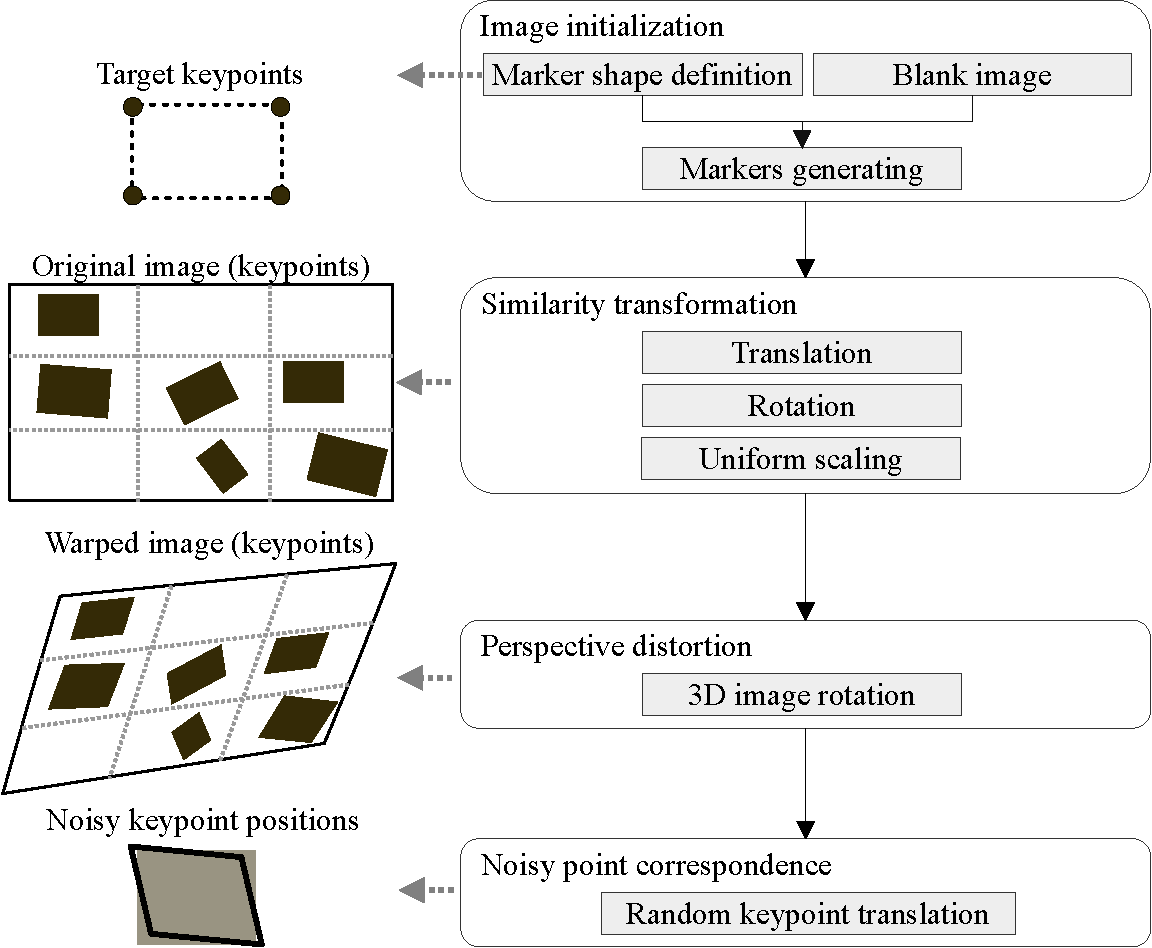
\includegraphics[width=0.7\linewidth]{figures/homography/dataset_generating.pdf}
    \caption[Description of creation of test scenarios]{Description of how each one of $t$ test instances in a specific test scenario is created. The input is a blank $w \times h$ image over which $m$ markers are initialized in a uniform grid, which produces the original marker keypoints. Depending on the test scenario, a particular subset of similarity transformations is applied to the entire image. Subsequently, warped keypoints are modified by random noise to simulate noisy point correspondence.}
    \label{fig:DatasetGenerating}
\end{figure}
% ------------------------------------------------------------------------------

% ##############################################################################
\subsection{Evaluation Methodology}
\label{ssec:evaluation_methodology}

\subsubsection{Error Computation}
\label{sssec:error_computation}

\def\warpedpix{\vect{w}}
\def\origpix{\vect{g}}

The accuracy of the developed method was evaluated by measuring the reprojection error using the Euclidean distance between the original and the rectified pixel positions. To obtain an error over the entire image, we computed the error for each pixel. Specifically, let $w$ and $h$ be the width and height of the image, respectively. The $3$D rotation of a point in the image around the image center that produces perspective distortion is represented by $\func{\varphi}{\cdot}$. Let $\subsup{\origpix}{i,j}{T} = \sbrackets{j, i, 1}$ be the original (ground-truth) pixel position at the $i$-th row and $j$-th column, and let $\warpedpix_{i, j} = \func{\varphi}{\origpix_{i, j}}$ be the analogically defined warped pixel position, for $i = 1, \dots, h, j = 1, \dots, w$. We then compute the $2$D reprojection error grid (a $h \times w$ matrix) for the given homography $\H$ as
\begin{equation}
    \label{eq:reprojection_error_grid}
    \boldsymbol{\xi}_{wh} =
    \begin{bmatrix}
        \func{e}{\warpedpix_{1, 1}, \origpix_{1, 1}} & \dots & \func{e}{\warpedpix_{1, w}, \origpix_{1, w}} \\
        \dots                                        & \dots & \dots                                        \\
        \func{e}{\warpedpix_{h, 1}, \origpix_{h, 1}} & \dots & \func{e}{\warpedpix_{h, w}, \origpix_{h, w}}
    \end{bmatrix},
\end{equation}
where
\begin{equation}
    \func{e}{\warpedpix, \origpix} = \euclnorm{\H \warpedpix - \origpix}.
\end{equation}
To simply express the reprojection error as a single number for the whole image, we adopted an arithmetic mean of all the values in the error grid above, so
\begin{equation}
    \label{eq:ReprojectionErrorSingle}
    \xi_{\text{reproj}} =
    \frac{1}{wh}
    \sum_{i = 1}^{h}
    \sum_{j = 1}^{w}
    \func{e}{\warpedpix_{i, j}, \origpix_{i, j}}.
\end{equation}

\subsubsection{Evaluation Algorithm}
\label{sssec:EvaluationAlgorithm}

On the input, there are $m$ markers (\sectiontext{}~\ref{ssec:HomographyDatasetCreation}) and thus an $m$-to-$1$ point correspondence. Each marker, by definition, provides a unique homography. Therefore, the aim is to quantify the relative improvement in the reprojection error over the baseline when the $k$-th ranked homography is used for rectification. Even though we are primarily concerned only with the single, top-performing homography, we evaluate the entire ranking to demonstrate its stable behavior.

We evaluated our homography ranking in terms of reprojection error improvements against the existing approaches based on the isolated homography estimation represented by implementation from the \opencv{}~\cite{bradski2008learning} library. Since our method provides a ranking, we compare our performance against a random marker selection based on uniform probability distribution. We refer to this performance as the ``baseline''; an unbiased marker selection. In practice, the user would rely on ``educated guess'' when predicting which marker could potentially be the best one to use. To obtain the aforementioned baseline, we evaluated the reprojection error \ref{eq:ReprojectionErrorSingle} for each marker in isolation and computed the arithmetic mean of these values. When we executed our proposed algorithm, we got the full ordering of markers by their score value computed using the proposed criterion \ref{eq:HomographyScoreFunction}. We expected that if the first marker were used to rectify the image, then the reprojection error would be minimal (and lower than the baseline error). If any subsequent marker in the given order were used instead, the reprojection error would increase.

We computed the relative improvement in \% for each $k$-th homography according to the baseline performance. Each test scenario was evaluated one by one. For each test instance, we obtained a $k$-dimensional vector where its elements represented a percentual improvement at each $k$-th position. We represented our data as a $t \times k$ matrix, where $t$ was the number of test instances. We treated each column independently to compute the statistics. The details of our evaluation algorithm are described in Algorithm~\ref{alg:EvaluationAlgorithm}. For simplicity, we show an evaluation of just a single instance.

\def\meanerrs{\boldsymbol{e}}
\def\errdiffs{\boldsymbol{p}}
\def\arracc{\left[ \right]}

\begin{algorithm}[t]
    \caption[Homography ranking evaluation algorithm]{Homography ranking evaluation algorithm.}
    \label{alg:EvaluationAlgorithm}
    \begin{algorithmic}[1]
        \State $\hmatrices, \sortres \gets $ \Call{rankhomographies}{\ }
        \Comment{apply homography ranking (\algtext{}~\ref{alg:HomographyRanking})}

        \State $e_b \gets 0$
        \Comment{baseline error, initially zero due to summation}

        \State $\meanerrs \gets \arraydef \left[ m \right]$
        \Comment{empty array to store reprojection errors}

        \State $\errdiffs \gets \arraydef \left[ m \right]$
        \Comment{empty array to store relative improvements}

        \For{$i \gets 1, \dots , m$}
        \Comment{for each marker}

        \State $\meanerrs \left[ i \right] \gets $ $\xi_{\text{reproj}}$
        \Comment{compute reprojection error (\eqtext{}~\ref{eq:ReprojectionErrorSingle})}

        \State $e_b \gets e_b + \meanerrs \left[ i \right]$
        \Comment{update baseline error}
        \EndFor

        \State $e_b \gets e_b / m$
        \Comment{compute the mean reprojection error}

        \For{$i \gets 1, \dots , m$}
        \Comment{for each marker}

        \State $k \gets \sortres \left[ i \right]$
        \Comment{position of $i$-th best homography}

        \State $\errdiffs \left[ i \right] \gets \rbrackets{e_b - \meanerrs \left[ k \right]} / e_b$
        \Comment{compute the relative improvement}
        \EndFor

        \State \Return $\errdiffs$
        \Comment{return the array of relative improvements}
    \end{algorithmic}
\end{algorithm}

% ##############################################################################
\subsection{Experimental Results}
\label{ssec:EvaluationResults}

\figtext{}~\ref{fig:HeatmapsBestWorst} shows how the reprojection error varies with respect to the marker position. We can see that the marker position can be deduced by looking at the heatmap representing the pixel-wise reprojection error over the image. The transformation achieves the best accuracy in the marker neighborhood and steadily decreases for more distant pixels. However, not all markers are subjected to the same pattern of error variation. This observation was the core motivation for our solution. We aim to choose the marker that minimizes the pixel-wise reprojection error within the region of the image that is as broad as possible. That is why we evaluate our method by computing the reprojection error over each pixel, not just the keypoints.

All tested scenarios depict similar trends as shown on the plots in \figtext{}~\ref{fig:SimilarityTransformInfluence}, \figtext{}~\ref{fig:NoiseInfluence}, \figtext{}~\ref{fig:ShapeInfluence} and in \figtext{}~\ref{fig:NMarkersInfluence}. The box plots extend from the lower to upper quartile values, with the thin and thick lines representing the median and mean, respectively. The plots discussed further show relative improvements over the baseline \opencv{}~\cite{bradski2008learning} method. We evaluated relative improvements for the sake of interpretability. For better comprehension, we suggest to see \tabletext{}~\ref{tab:TestScenariosResults}. It contains individual test scenarios and their corresponding top performances in percents. Conversely, the reprojection error in absolute terms is difficult to interpret without additional context. Nevertheless, to highlight the differences in reprojection errors we also provide absolute values in \tabletext{}~\ref{tab:TestScenariosResults}. The presence of noise shifted the errors by multiple magnitudes, but still preserved the pattern of distribution.

\subsubsection{Influence of Similarity Transformations}

In this test scenario, we tested in isolation each allowed similarity transformation, \ietext{}, translation, rotation, and uniform scaling. \figtext{}~\ref{fig:SimilarityTransformInfluence} demonstrates that the relative improvement was circa equal in all situations. Besides, we show that the proposed method is practically invariant to similarity transformations allowing the markers to be in arbitrary positions in a plane. When all similarity transformations were utilized, our method performed even better, showing its stability and robustness.

\def\boxplotimgwidth{0.75\linewidth}

% ------------------------------------------------------------------------------
\begin{figure}[t]
    \centering
    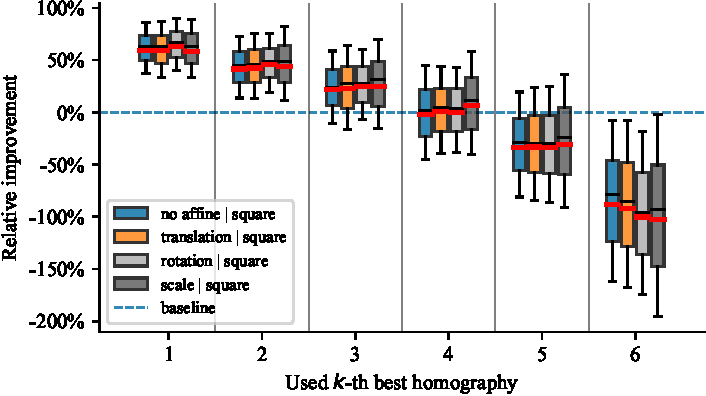
\includegraphics[width=\boxplotimgwidth]{figures/homography/similarity_transform_influence.pdf}
    \caption[Influence of similarity transformation]{Influence of similarity transformation on the reprojection error.}
    \label{fig:SimilarityTransformInfluence}
\end{figure}
% ------------------------------------------------------------------------------

\subsubsection{Influence of Noise}

In \figtext{}~\ref{fig:NoiseInfluence}, we can see the effect of noisy point correspondence that simulated inaccurate keypoint detection. The ranking method preserved the trend of the relative improvement in presence of noise. Absolute reprojection error demonstrated that unless noise was present, the errors varied on sub-pixel levels, so they were practically zero.

% ------------------------------------------------------------------------------
\begin{figure}[t]
    \centering
    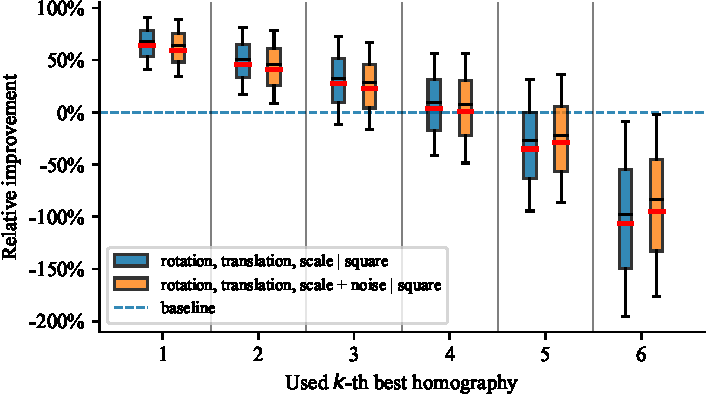
\includegraphics[width=\boxplotimgwidth]{figures/homography/noise_influence.pdf}
    \caption[Influence of noise]{Influence of noise applied to the warped keypoints representing a noisy point correspondence.}
    \label{fig:NoiseInfluence}
\end{figure}
% ------------------------------------------------------------------------------

\subsubsection{Influence of Variable Shapes}

We expected that the relative improvement of our method should be invariant to variable shapes as long as they were similar. \figtext{}~\ref{fig:ShapeInfluence} demonstrates that with an increasing number of keypoints our method consistently preserved its capabilities. Introducing more complicated shapes than just rectangles did not exacerbate the outcome of the algorithm.

% ------------------------------------------------------------------------------
\begin{figure}[t]
    \centering
    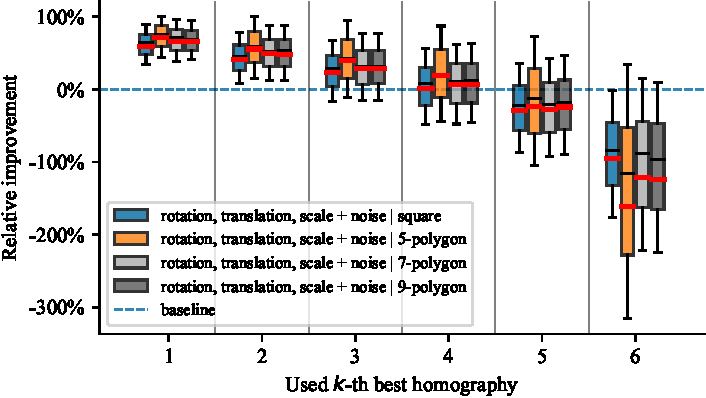
\includegraphics[width=\boxplotimgwidth]{figures/homography/shape_influence.pdf}
    \caption[Influence of marker shape]{Results for different marker shapes.}
    \label{fig:ShapeInfluence}
\end{figure}
% ------------------------------------------------------------------------------

\subsubsection{Influence of Number of Markers}

We tested a variable number of markers to demonstrate that our method preserved its improvement. \figtext{}~\ref{fig:NMarkersInfluence} shows that the greater the set of markers, the better the relative improvement. Even when we used just three markers, the proposed method achieved a $46.91$\% median relative improvement. While it is beneficial to use a larger number of markers, we believe that the improvement we can obtain from an increasing number of markers has a logarithmic trend. On the extreme side, if we used only one marker, there would be no improvement since there would be only one homography to choose from.

\begin{figure*}[t]
    \centering
    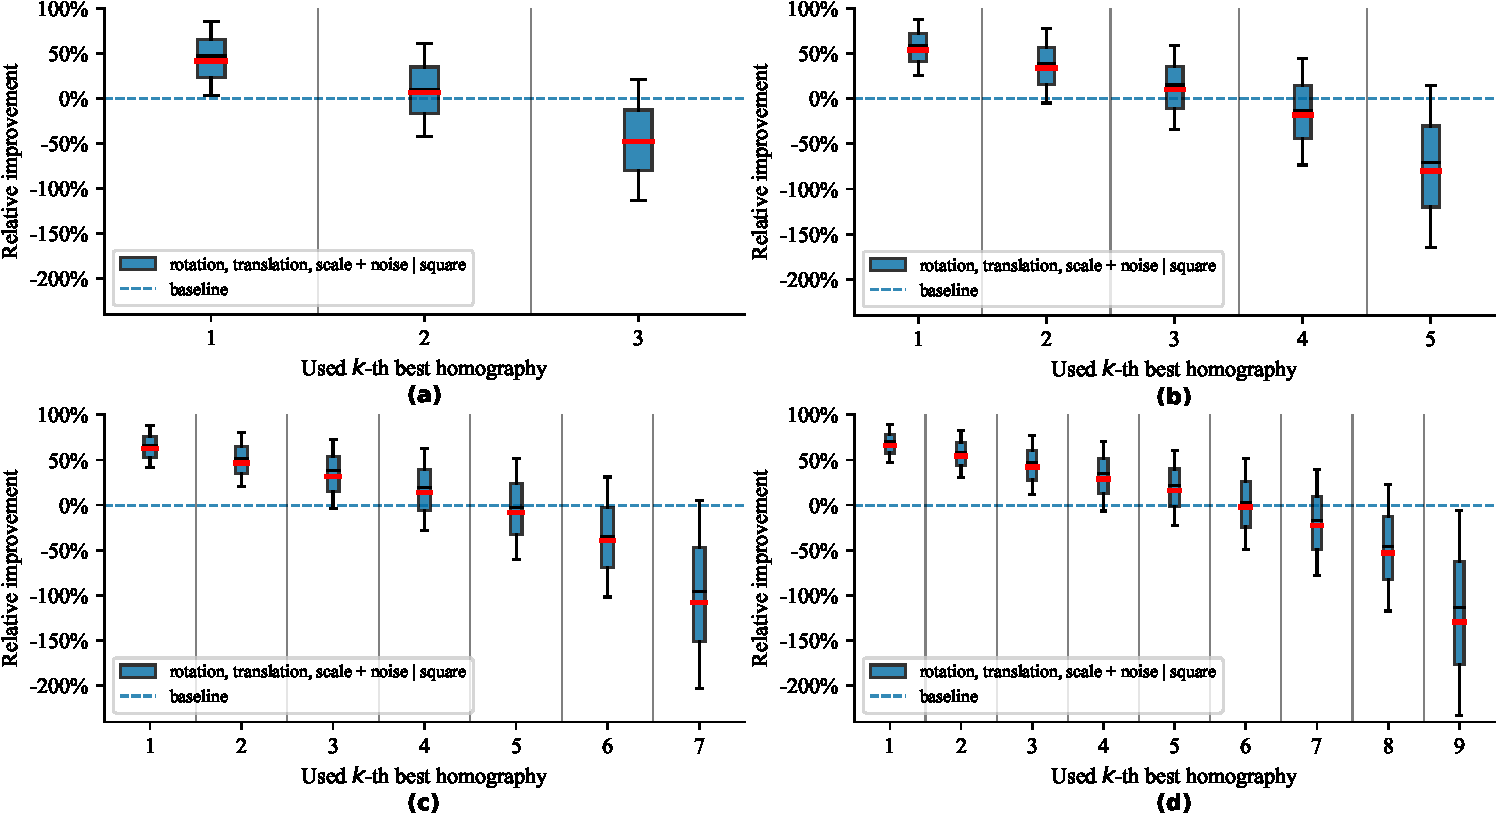
\includegraphics[width=\linewidth]{figures/homography/n_markers_influence.pdf}
    \caption[Influence of number of markers]{Influence of different number of markers on reprojection error. We experimented with \imgpartdesc{a} three, \imgpartdesc{b} five, \imgpartdesc{c} seven, and \imgpartdesc{d} nine markers.}
    \label{fig:NMarkersInfluence}
\end{figure*}

\def\tblsccolw{0.06}
\def\tblrscolw{0.08}
\begin{table*}[t]
    \caption[Description of synthetic dataset scenarios]{Description of test scenarios in our synthetic dataset with corresponding settings and results for the top-ranked homography. One row represents one test scenario. Four visually separated groups (from top to bottom) are related to experiments shown in \figtext{}~\ref{fig:SimilarityTransformInfluence}~-~\ref{fig:NMarkersInfluence}.}
    \label{tab:TestScenariosResults}
    \setlength{\tabcolsep}{3pt}
    \begin{center}
        \footnotesize
        \begin{tabular}{p{\tblsccolw\linewidth}p{0.03\linewidth}p{\tblsccolw\linewidth}p{\tblsccolw\linewidth}p{\tblsccolw\linewidth}p{\tblsccolw\linewidth}|p{\tblrscolw\linewidth}p{\tblrscolw\linewidth}p{\tblrscolw\linewidth}p{\tblrscolw\linewidth}p{\tblrscolw\linewidth}p{\tblrscolw\linewidth}}
            \toprule
            \multirow{2}{2pt}{\textbf{shape}}  &
            \multirow{2}{2pt}{\textbf{\#}}     &
            \multirow{2}{2pt}{\textbf{trans.}} &
            \multirow{2}{2pt}{\textbf{rot.}}   &
            \multirow{2}{2pt}{\textbf{scale}}  &
            \multirow{2}{2pt}{\textbf{noise}}  & \multicolumn{3}{l}{\textbf{relative improvement}} & \multicolumn{3}{l}{\textbf{absolute improvement}}                                                                                                      \\
                                               &                                                   &                                                   &     &     &     & \textbf{median} & \textbf{mean} & \textbf{stdev} &
            \textbf{median}                    & \textbf{mean}                                     & \textbf{stdev}                                                                                                                                         \\
            \midrule
            square                             & 6                                                 & no                                                & no  & no  & no  & 62.80\%         & 59.63\%       & 19.64\%        & 0.0003  & 0.0003   & 0.0001   \\
            square                             & 6                                                 & yes                                               & no  & no  & no  & 62.65\%         & 59.00\%       & 19.72\%        & 0.0003  & 0.0003   & 0.0001   \\
            square                             & 6                                                 & no                                                & yes & no  & no  & 66.42\%         & 63.17\%       & 19.11\%        & 0.0004  & 0.0004   & 0.0002   \\
            square                             & 6                                                 & no                                                & no  & yes & no  & 63.38\%         & 58.51\%       & 23.97\%        & 0.0002  & 0.0003   & 0.0002   \\
            \midrule
            square                             & 6                                                 & yes                                               & yes & yes & no  & 67.82\%         & 63.66\%       & 20.30\%        & 0.0004  & 0.0004   & 0.0002   \\
            square                             & 6                                                 & yes                                               & yes & yes & yes & 64.11\%         & 59.26\%       & 22.12\%        & 22.0781 & 24.3177  & 15.0085  \\
            \midrule
            5-poly                             & 6                                                 & yes                                               & yes & yes & yes & 74.67\%         & 71.19\%       & 21.98\%        & 69.5553 & 336.2653 & 685.7427 \\
            7-poly                             & 6                                                 & yes                                               & yes & yes & yes & 71.02\%         & 65.63\%       & 22.99\%        & 46.7939 & 135.6574 & 395.7526 \\
            9-poly                             & 6                                                 & yes                                               & yes & yes & yes & 68.97\%         & 65.57\%       & 21.98\%        & 44.9763 & 115.1219 & 309.2720 \\
            \midrule
            square                             & 3                                                 & yes                                               & yes & yes & yes & 46.91\%         & 41.36\%       & 31.58\%        & 14.7750 & 18.1155  & 20.6746  \\
            square                             & 5                                                 & yes                                               & yes & yes & yes & 59.03\%         & 53.91\%       & 24.56\%        & 19.7629 & 22.5333  & 16.0080  \\
            square                             & 7                                                 & yes                                               & yes & yes & yes & 66.19\%         & 62.41\%       & 19.98\%        & 23.8768 & 27.1364  & 32.2853  \\
            square                             & 9                                                 & yes                                               & yes & yes & yes & 69.86\%         & 66.09\%       & 18.18\%        & 25.6645 & 26.6838  & 11.6975  \\
            \bottomrule
        \end{tabular}
    \end{center}
\end{table*}
\section{Conclusion}

In this homography-related subpart of our object tracking research, we proposed a method that builds on top of existing approaches for homography estimation that utilize existing point correspondences. The method is a systematic ranking of a set of homography matrices while exploiting the proposed score function to establish the order. Each homography in such a set belongs to a specific marker.

We consistently demonstrated that the proposed solution is robust in presence of noise in the point correspondences. These correspondences can be either algorithmically found using feature-matching algorithms (\egtext{}, \gls{sift}~\cite{lowel1999objrecognition}) or annotated manually, but one has to keep in mind that even human annotations are often inaccurate. We also showed the robustness of our method to a varying number of markers and a change in shape.

Generally speaking, all the improvements at individual ranking positions steadily decreased, reaching $0$\% improvement at around $\nicefrac{2}{3}~m$, where $m$ is the number of markers. A practically applicable statement would be the following: ``the first half of ranked homographies yields a better reprojection compared to the baseline on average.''. The baseline performance was given by an average \opencv{}~\cite{bradski2008learning} reprojection error under the assumption of no prior preference of specific markers, hence the random marker selection.

A practical advantage of our algorithm is that it is invariant to the underlying homography estimation method. It can, therefore, serve as an extension to all existing or future approaches that handle point correspondences, either as part of run time or a post-processing stage. Moreover, it is computationally very efficient, as it scales well with a quadratic complexity $\func{\Theta}{m^2}$ in the number of markers, which is usually a single-digit number.

The proposed homography ranking found a real-world application within our solution for the university-related \interreg{} project where we tackled the problem of tracking vehicles for the purpose of speed and dimension estimation. Homography mapping was a necessary part of our approach. However, we did not continue with this branch of research due to the lack of available datasets that we would require for a deep learning-based object tracking solution involving perspective projections.

